% Drawing 154/08-3 -- folder 154, batch 08, archive page 143 (PDF page 144).
% Transcription: croquis au crayon et à l'encre, sans texte : des arrangements de trois ou quatre droites qui se coupent, certaines en étoile autour d'un point ; à gauche et à droite, des chemins en tirets (bruns, verts) qui longent un segment épais entre deux croisements
% Kind: pencil and ink arrangements of three or four lines, stars round a point; dashed paths along a thick segment. Method 2 (schematic redraw from the facsimile). Status: partial.
% Notes: Pencil and ink sketches without text over a job banner (not reproduced), read from the page view: arrangements of three or four lines that cut one another, some in a star round a point; at the left and the right, dashed paths (brown, green) running along a thick segment between two crossings. Lines placed approximately.
% Coordinates: 1 unit = 1 mm = 1/100 of the crop width (bbox in page fractions: [0.107, 0.082, 0.964, 0.265]).
% Redrawn by Claude (claude-opus-5-5), issue #73, 2026-11-07; not checked by a human; not compiled (no TeX in the session).
% Rights: reproduces part of the work -- behind RENDER_TRANSCRIPTS, never published by itself.
\documentclass[tikz,border=3pt]{standalone}
\usepackage{amsmath,amssymb}
\usetikzlibrary{patterns,arrows.meta}
\tikzset{Or/.style={orange!90!black}, Ye/.style={yellow!80!orange}, Lg/.style={green!60!black!70}, Dg/.style={green!45!black}, Br/.style={brown!80!black}, Rd/.style={red!85!black}, Bl/.style={blue!70!black}, Gy/.style={black!40}, pencil/.style={black!45}, struck/.style={black!35}, mark/.style={circle,draw,inner sep=1.3pt}, pt/.style={circle,fill,inner sep=0.9pt}, opt/.style={circle,draw,fill=white,inner sep=1.1pt}}
\begin{document}
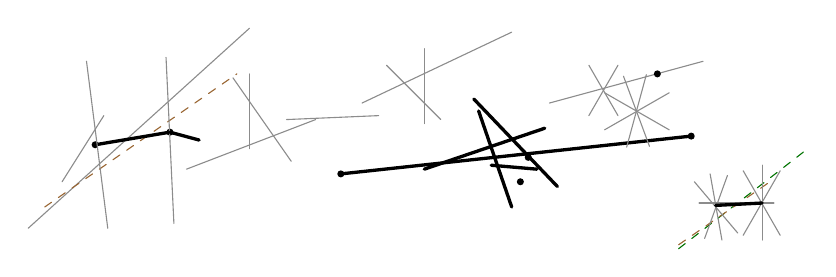
\begin{tikzpicture}[x=1mm,y=1mm,line cap=round,line join=round,font=\scriptsize]
\draw[pencil] (0.5,-26.5) -- (28.6,-1.1);
\draw[Br,dashed] (2.6,-23.8) -- (27,-6.9);
\draw[very thick] (9,-15.9) -- (18.5,-14.3);
\node[pt] at (9,-15.9) {};
\node[pt] at (18.5,-14.3) {};
\draw[pencil] (7.9,-5.3) -- (10.6,-26.5);
\draw[pencil] (18,-4.8) -- (19,-25.9);
\draw[pencil] (4.8,-20.6) -- (10.1,-12.2);
\draw[very thick] (18.5,-14.3) -- (22.2,-15.3);
\draw[pencil] (26.5,-7.4) -- (33.9,-18);
\draw[pencil] (28.6,-6.9) -- (28.6,-16.4);
\draw[pencil] (20.6,-19) -- (37,-12.7);
\draw[very thick] (40.2,-19.6) -- (84.7,-14.8);
\node[pt] at (40.2,-19.6) {};
\node[pt] at (84.7,-14.8) {};
\node[pt] at (64,-17.5) {};
\node[pt] at (63,-20.6) {};
\draw[very thick] (57.1,-10.1) -- (67.7,-21.2);
\draw[very thick] (66.1,-13.8) -- (50.8,-19);
\draw[very thick] (57.7,-11.6) -- (61.9,-23.8);
\draw[very thick] (59.3,-18.5) -- (65.1,-19);
\draw[pencil] (42.9,-10.6) -- (61.9,-1.6);
\draw[pencil] (50.8,-3.7) -- (50.8,-13.2);
\draw[pencil] (46,-5.8) -- (52.9,-12.7);
\draw[pencil] (33.3,-12.7) -- (45,-12.2);
\draw[pencil] (66.7,-10.6) -- (86.2,-5.3);
\draw[pencil] (73.7,-14) -- (81.9,-9.3);
\draw[pencil] (76.5,-16.2) -- (79,-7);
\draw[pencil] (79.4,-16.1) -- (76.1,-7.2);
\draw[pencil] (81.9,-14) -- (73.7,-9.3);
\node[pt] at (80.4,-6.9) {};
\draw[pencil] (71.7,-12.2) -- (75.4,-5.8);
\draw[pencil] (75.4,-12.2) -- (71.7,-5.8);
\draw[Dg,dashed] (83.1,-29.1) -- (99.5,-16.4);
\draw[Br,dashed] (83.1,-28.6) -- (94.7,-20.6);
\draw[pencil] (85.7,-23.3) -- (95.2,-23.3);
\draw[pencil] (86.4,-27.8) -- (89.3,-19.8);
\draw[pencil] (88.6,-28) -- (87.1,-19.6);
\draw[pencil] (90.6,-27.1) -- (85.1,-20.6);
\draw[pencil] (91.3,-27.4) -- (96,-19.2);
\draw[pencil] (93.7,-28) -- (93.7,-18.5);
\draw[pencil] (96,-27.4) -- (91.3,-19.2);
\draw[very thick] (87.8,-23.6) -- (93.7,-23.3);
\end{tikzpicture}
\end{document}
